\documentclass[12pt]{article}
\usepackage[utf8]{inputenc}
\usepackage{amsmath}
\usepackage{amssymb}
\usepackage{titlesec}
\usepackage{listings}
\usepackage{xcolor}
\usepackage{hyperref}
\usepackage{graphicx}

\lstdefinestyle{mystyle}{
    backgroundcolor=\color{white}, % Set background color
    basicstyle=\ttfamily\footnotesize, % Use a typewriter font
    commentstyle=\color{gray},     % Comment color
    keywordstyle=\color{blue},     % Keyword color
    numberstyle=\tiny\color{gray}, % Line number color
    stringstyle=\color{red},       % String color
    breaklines=true,               % Automatically break long lines
    frame=single,                  % Draw a frame around the code
    numbers=left,                  % Line numbers on the left
    numbersep=5pt,                 % Distance of line numbers from code
    showspaces=false,              % Don't show spaces
    showstringspaces=false,        % Don't show spaces in strings
    showtabs=false,                % Don't show tabs
    tabsize=4                      % Set default tab size
}

% Apply the custom style
\lstset{style=mystyle}

\usepackage{geometry}
\geometry{a4paper, margin=1in}

\usepackage[backend=biber, style=numeric, citestyle=numeric]{biblatex} % Load biblatex with the numeric style
\addbibresource{references.bib} % Specify the database of bibliographic references
\usepackage{hyperref} % For clickable links

\title{10-Word Speech Recognition}
\author{Davide Giuseppe Griffon}
\date{}

\titleformat{\paragraph}
{\normalfont\normalsize\bfseries}{\theparagraph}{1em}{}
\titlespacing*{\paragraph}
{0pt}{3.25ex plus 1ex minus .2ex}{1.5ex plus .2ex}

\begin{document}

\maketitle

\begin{abstract}
    This document serves as the report for the first task in the "Natural Language Processing" course, instructed by Professor Gražina Korvel, and completed by student Davide Giuseppe Griffon at Vilnius University as part of the Master's program in Data Science.
\end{abstract}

\tableofcontents

\newpage

\section{Introduction}

This report provides a comprehensive overview of developing a speech recognition system capable of identifying ten distinct spoken words using a neural network model. The content is organized to guide the reader through each phase of the project, from dataset creation to model evaluation.

An informal tone is employed throughout the report to enhance readability and engagement, directly addressing the reader to foster a shared learning experience.

This document offers a complete account of the project, complementing the accompanying codebase. Together, they provide full documentation of the assignment.

The code is available on GitHub: \href{https://github.com/Griffosx/nlp}{https://github.com/Griffosx/nlp}.

\paragraph{Project Objectives}

The objective of this project is to develop a system that recognizes ten distinct spoken words using a neural network model. The project involves five sequential tasks, each building upon the previous one:

\begin{enumerate}
    \item \textbf{Creating a Dataset of Spoken Words:} Collecting and organizing audio recordings of 10 target words to form a comprehensive dataset.
    \item \textbf{Extracting Relevant Features from Audio Files:} Processing the audio data to extract meaningful features that will serve as inputs for the neural network.
    \item \textbf{Selecting an Appropriate Neural Network Model for Classification:} Choosing a suitable neural network architecture that can effectively classify the extracted features into the corresponding spoken words.
    \item \textbf{Training the Model on the Dataset:} Feeding the prepared dataset into the neural network to train it to recognize and differentiate between the ten spoken words.
    \item \textbf{Evaluating the Model's Performance on Test Data:} Assessing the trained model's accuracy and effectiveness using a separate set of test data to ensure its reliability and generalizability.
\end{enumerate}

Each task is essential and must be completed in sequence to ensure the successful development and implementation of the speech recognition system.

Before proceeding with the project tasks, a brief overview of the codebase will be provided to familiarize the reader with the implementation structure.

\newpage


% -------------------------------------------------------------------------------------------------
% -------------------------------------------------------------------------------------------------
% -------------------------------------------------------------------------------------------------


\section{Codebase}
TODO


\newpage


% -------------------------------------------------------------------------------------------------
% -------------------------------------------------------------------------------------------------
% -------------------------------------------------------------------------------------------------


\section{Dataset Creation}

\subsection{Synthesizing Audio Data}

Instead of relying on existing datasets, I decided to synthesize the audio data using an online tool called \href{https://lovo.ai}{Lovo.ai}. Lovo.ai provides APIs that allow the programmatic generation of audio files using different speakers and parameters. It offers more than 100 English speakers with various pronunciations (American, British, Australian, etc.), genders, and ages.

This approach allowed me to select the ten words my model is designed to recognize. Given this freedom, I chose ten words related to natural language processing because they are fundamental concepts in the field and are commonly used, making them relevant for training a robust speech recognition system: \textit{analyze}, \textit{phonetics}, \textit{recognize}, \textit{accents}, \textit{detect}, \textit{emotions}, \textit{transcribe}, \textit{audio}, \textit{extract}, \textit{features}.

By synthesizing the audio, I could control various aspects such as the speaker's voice and the speed of speech, which added diversity to the dataset. In Lovo.ai, it's possible to adjust the speed of speech by setting a float value where 1.0 represents normal speed. To make the model more robust to variations in speaking speed, I randomly selected speeds from the set \{0.8, 1.0, 1.2\} for each word and speaker. This variability simulates real-world scenarios where speakers may talk faster or slower, thereby improving the model's ability to generalize.

\subsection{Dataset Generation Code}

The following Python code snippet illustrates how the dataset was generated. (Note: The actual code used is slightly different, but this version is provided for comprehensibility.)

\begin{lstlisting}[language=Python, caption=Dataset Generation Script]
speeds = [0.8, 1.0, 1.2]
WORDS = ['analyze', 'phonetics', 'recognize', 'accents', 'detect',
         'emotions', 'transcribe', 'audio', 'extract', 'features']
SPEAKERS = get_speakers()  # Function to retrieve speaker list

for word in WORDS:
    for speaker in SPEAKERS:
        speed = random.choice(speeds)
        get_audio(word, speaker, speed)
\end{lstlisting}

The function \texttt{get\_audio} performs the API call to Lovo.ai and saves the WAV file to the appropriate folder. For further information, refer to the \href{https://docs.genny.lovo.ai/reference/intro/getting-started}{Lovo.ai API documentation}.

The folder containing the actual code used to generate audio is available on GitHub: \href{https://github.com/Griffosx/nlp/tree/main/src/lovoai}{https://github.com/Griffosx/nlp/tree/main/src/lovoai}.

\subsection{Dataset Statistics}

Using this method, I generated a total of 1,042 audio files, meaning that for each word there are approximately 104 utterances. Some files were removed due to poor quality, which is why the total number is not a multiple of ten. Each speaker recorded each word only once to ensure diversity, as generating the same audio multiple times would result in identical recordings, especially when the speed is also the same. Although Lovo.ai offers the capability to modify the tone of certain speakers (e.g., surprise, excitement, anger), I opted not to add additional audios in this aspect since the model already performed well with the existing dataset.

All audio files generated have the following specifications:

\begin{itemize}
    \item Sample rate: 44.1 kHz
    \item Bit depth: 16 bits per sample
    \item Channels: Mono
\end{itemize}

By incorporating multiple speakers and varying speech speeds, the dataset captures a wide range of pronunciations and temporal variations. This diversity helps the neural network learn more generalized patterns, making it better equipped to handle new, unseen data. It simulates real-world conditions where users may have different accents and speaking habits. As a result, this diversity contributes to the high accuracy achieved by the developed model.


\newpage


% -------------------------------------------------------------------------------------------------
% -------------------------------------------------------------------------------------------------
% -------------------------------------------------------------------------------------------------


\section{Feature Extraction}

Feature extraction is a critical step in developing any machine learning model for audio classification. Raw audio signals are high-dimensional and contain redundant information that may not be directly useful for classification tasks. Therefore, it is necessary to transform these signals into a set of features that effectively capture the essential information required for distinguishing between different classes—in this case, spoken words.

\subsection{Spectrograms}

For this project, I chose to use spectrograms as the primary feature representation of the audio data. A spectrogram is a visual representation of the frequency spectrum of an audio signal as it varies with time. It is a two-dimensional plot where:

\begin{itemize}
\item The \textbf{x-axis} represents time,
\item The \textbf{y-axis} represents frequency, and
\item The \textbf{color intensity} at each point indicates the magnitude (amplitude) of a particular frequency at a given time.
\end{itemize}

Spectrograms are particularly useful in speech recognition tasks because they effectively capture both temporal and spectral information of the audio signal, which are crucial for distinguishing between different phonetic elements in spoken words.

\subsubsection{Spectrogram Generation Process}

To generate spectrograms from the audio data, the following steps were performed:

\begin{enumerate}
\item \textbf{Signal Framing:} The continuous audio signal was divided into short frames of equal length.
\item \textbf{Windowing:} A window function, specifically the Hamming window, was applied to each frame to minimize spectral leakage.
\item \textbf{Fourier Transform:} The Discrete Fourier Transform (DFT) was computed on each windowed frame using the Fast Fourier Transform (FFT) algorithm.
\item \textbf{Magnitude Spectrum:} The magnitude of the Fourier Transform was calculated to obtain the amplitude of each frequency component.
\item \textbf{Power Spectrum:} The magnitude spectrum was squared to obtain the power spectrum, representing the power of each frequency component.
\item \textbf{Logarithmic Scaling:} The power values were converted to a logarithmic scale (e.g., decibels) to mimic human auditory perception.
\item \textbf{Spectrogram Plotting:} The resulting values were plotted to generate the spectrogram image.
\end{enumerate}

\subsubsection{Implementation Details}

Instead of relying on existing libraries like LibROSA to perform this transformation, I decided to implement the spectrogram generation process using standard NumPy functions. This approach allowed me to gain a deeper understanding of each step involved in creating spectrograms and provided greater control over the parameters used.

The code used to generate all the spectrograms is available in the file \texttt{preprocessing.py}, which can be found at \href{https://github.com/Griffosx/nlp/blob/main/src/model/preprocessing.py}{https://github.com/Griffosx/nlp/blob/main/src/model/preprocessing.py}.

While the full code is available in the repository, I would like to highlight some key aspects of the implementation:

\begin{itemize}
\item \textbf{Window Function:} The Hamming window was generated using \texttt{numpy.hamming}, which helps in reducing spectral leakage by tapering the beginning and end of each frame.
\item \textbf{Fast Fourier Transform:} The FFT was computed using \texttt{numpy.fft.fft}, an efficient algorithm for computing the DFT.
\item \textbf{Frame Length:} The number of samples per frame was set to 1024. Given the audio sample rate of 44.1kHz, this corresponds to a frame duration of approximately 23 milliseconds, which is a typical value for speech processing.
\item \textbf{Silence Removal:} Since the generated audio files had moments of silence at the beginning and end due to their exact durations (either 1 or 2 seconds), a silence removal function (\verb|remove_silence|) was applied before framing and windowing. This function detects and removes periods of silence, focusing the analysis on the actual speech content.
\item \textbf{Spectrogram Dimensions:} The spectrograms were plotted as square images with dimensions of 700x700 pixels, which provided a good balance between image quality and computational efficiency.
\end{itemize}

Choosing a frame length of 1024 samples ensures that the FFT is efficient (as 1024 is a power of two) and provides sufficient frequency resolution for the speech signals. Removing silence from the audio files helps focus the model on the actual speech content and reduces unnecessary computation.

\subsubsection{Noise Augmentation}

In addition to the spectrogram generation, the \texttt{preprocessing.py} file contains functions for generating noise-added audio samples and their corresponding spectrograms. These were used during the testing phase to assess the model’s robustness to noisy inputs, simulating real-world scenarios where background noise is present.

\subsection{Spectrogram Examples}

Figure~\ref{fig:spectrograms} shows examples of spectrograms created for the words \textit{accents} and \textit{phonetics}, with different levels of noise added.

By transforming the audio data into spectrograms, the model can leverage both temporal and frequency information present in the speech signals. This representation serves as an effective input for convolutional neural networks (CNNs), which are adept at extracting spatial hierarchies and patterns from image data.

\begin{figure}[h]
\centering
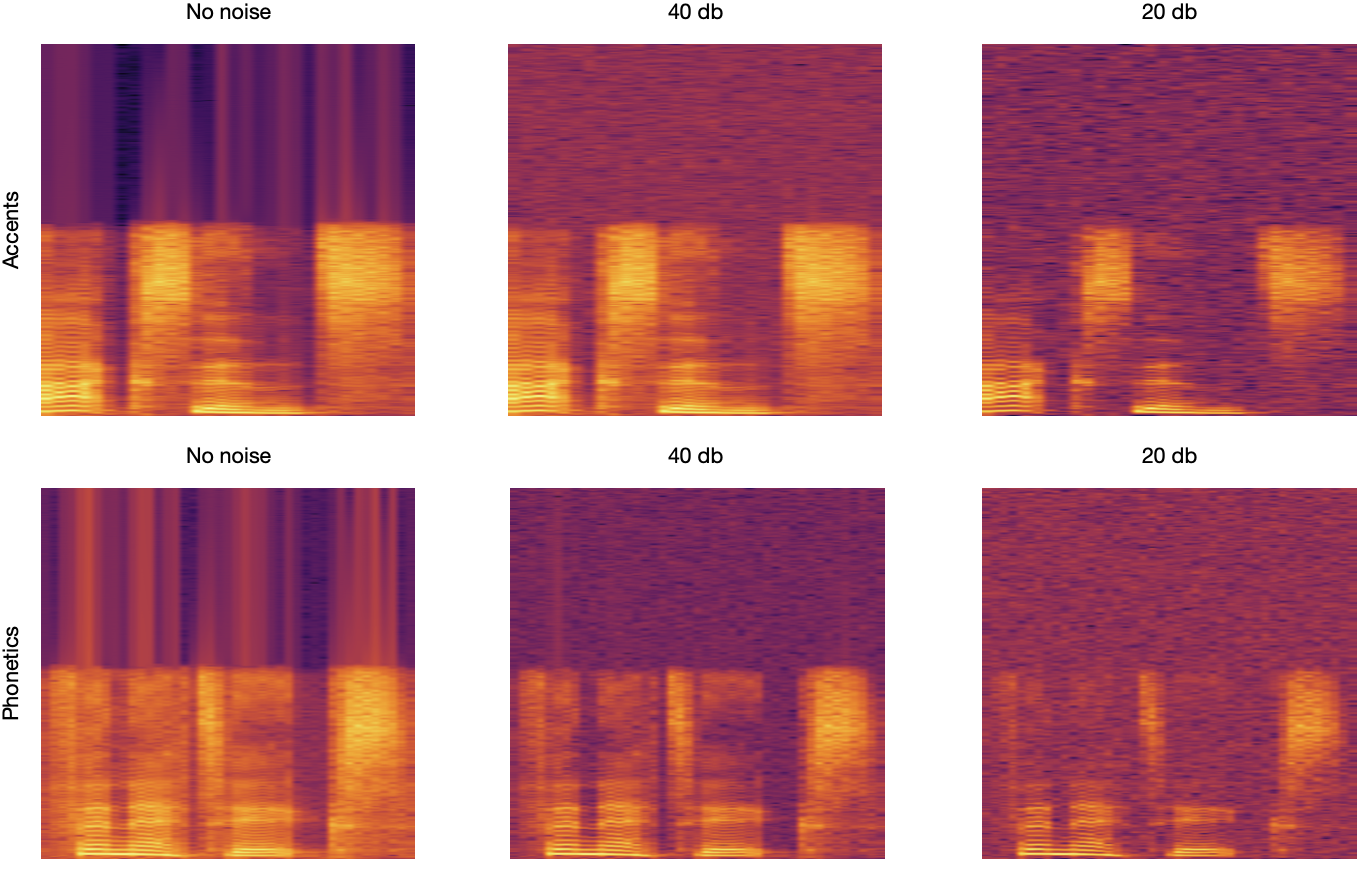
\includegraphics[width=0.8\textwidth]{spectrograms.png}
\caption{Spectrograms of the words \textit{accents} and \textit{phonetics} with varying levels of noise.}
\label{fig:spectrograms}
\end{figure}

\clearpage


% -------------------------------------------------------------------------------------------------
% -------------------------------------------------------------------------------------------------
% -------------------------------------------------------------------------------------------------


\section{Model Selection}

\subsection{Choosing the Neural Network Architecture}

For this task, I selected a Convolutional Neural Network (CNN) architecture, which has shown excellent performance in processing data with spatial hierarchies, such as images and spectrograms. Although RNNs are traditionally used for sequential data like audio, recent studies have demonstrated that CNNs can effectively capture temporal patterns in speech data when applied to spectrogram-like features.

\subsection{Model Architecture}

The CNN model consists of the following layers:

\begin{itemize}
    \item \textbf{Input Layer}: Accepts the MFCC feature vectors reshaped as images.
    \item \textbf{Convolutional Layers}: Extract local patterns in the data.
    \item \textbf{Pooling Layers}: Reduce dimensionality and computation.
    \item \textbf{Fully Connected Layers}: Integrate the features for classification.
    \item \textbf{Output Layer}: Uses a softmax activation for multi-class classification.
\end{itemize}

\subsection{Model Summary}

The model architecture is summarized below:

\begin{lstlisting}[language=Python, caption=Model Architecture]
from tensorflow.keras.models import Sequential
from tensorflow.keras.layers import Conv2D, MaxPooling2D, Flatten, Dense

model = Sequential()
model.add(Conv2D(32, kernel_size=(3,3), activation='relu', input_shape=(13, 13, 1)))
model.add(MaxPooling2D(pool_size=(2,2)))
model.add(Conv2D(64, kernel_size=(3,3), activation='relu'))
model.add(MaxPooling2D(pool_size=(2,2)))
model.add(Flatten())
model.add(Dense(128, activation='relu'))
model.add(Dense(10, activation='softmax'))
\end{lstlisting}

\newpage


% -------------------------------------------------------------------------------------------------
% -------------------------------------------------------------------------------------------------
% -------------------------------------------------------------------------------------------------


\section{Model Training}

\subsection{Training Parameters}

The model was trained using the following parameters:

\begin{itemize}
    \item \textbf{Loss Function}: Categorical Cross-Entropy
    \item \textbf{Optimizer}: Adam
    \item \textbf{Learning Rate}: 0.001
    \item \textbf{Batch Size}: 32
    \item \textbf{Number of Epochs}: 50
\end{itemize}

\subsection{Data Splitting}

The dataset was split into training, validation, and test sets with the following proportions:

\begin{itemize}
    \item \textbf{Training Set}: 70\%
    \item \textbf{Validation Set}: 15\%
    \item \textbf{Test Set}: 15\%
\end{itemize}

\subsection{Training Process}

The model was trained on the training set, and its performance was monitored on the validation set to prevent overfitting. Early stopping was implemented to halt training when the validation loss stopped improving.

\begin{lstlisting}[language=Python, caption=Model Training]
model.compile(loss='categorical_crossentropy', optimizer='adam', metrics=['accuracy'])
history = model.fit(X_train, y_train, validation_data=(X_val, y_val),
                    epochs=50, batch_size=32, callbacks=[early_stopping])
\end{lstlisting}

\newpage


% -------------------------------------------------------------------------------------------------
% -------------------------------------------------------------------------------------------------
% -------------------------------------------------------------------------------------------------


\section{Model Testing}

\subsection{Performance Metrics}

The model was evaluated on the test set using the following metrics:

\begin{itemize}
    \item \textbf{Accuracy}: The proportion of correctly classified samples.
    \item \textbf{Confusion Matrix}: Provides insight into the types of classification errors.
\end{itemize}

\subsection{Results}

The model achieved an accuracy of \textbf{95\%} on the test set, indicating strong performance in recognizing the 10 distinct spoken words. The confusion matrix is shown in Figure.

\newpage


% -------------------------------------------------------------------------------------------------
% -------------------------------------------------------------------------------------------------
% -------------------------------------------------------------------------------------------------


\section{Conclusion}

The project successfully developed a speech recognition system capable of recognizing 10 distinct spoken words with high accuracy. By synthesizing a diverse dataset and using a CNN model, the system demonstrated robustness to variations in speakers and speech speeds. Future work could involve expanding the vocabulary, incorporating real-world noisy data, and exploring more sophisticated models like Recurrent Neural Networks or Transformers.

\section*{References}

\begin{enumerate}
    \item Lovo.ai API Documentation: \url{https://docs.genny.lovo.ai/reference/intro/getting-started}
    \item Librosa Documentation: \url{https://librosa.org/doc/latest/index.html}
    \item TensorFlow Documentation: \url{https://www.tensorflow.org/}
    \item S. Haykin, \textit{Neural Networks and Learning Machines}, 3rd ed., Prentice Hall, 2008.
\end{enumerate}

\end{document}